\documentclass[french]{beamer}
\usepackage{comment}
\usepackage[utf8]{inputenc}
\usepackage[T1]{fontenc}
\usepackage{lmodern}
\usepackage{amsmath, amssymb}
\usepackage{multimedia}
\usepackage{babel}
\usepackage{subcaption}
\usepackage{pgfplots}
\usetheme[width=2cm]{PaloAlto}
\usepackage{graphicx}
\usepackage{textpos}
\usepackage{mathrsfs}
\usetikzlibrary{patterns}
\pgfplotsset{compat=1.15}
\usetikzlibrary{arrows}
\usepackage{multimedia}
\usepackage{pdfpages}
\usepackage{algorithm}
\usepackage{algorithmic}

\usepackage[backend=biber,style=numeric]{biblatex}
\addbibresource{bibliography/references.bib}

\title{Uncovering the structure of clinical EEG signals with self-supervised learning}
\subtitle{ Hubert Banville, Omar Chehab, Aapo Hyvärinen, Densi-Alexander Engemann and Alexandre Gramfort}
\author{ Romane Barra \\  Grégoire Béchade}
\date{8 Janvier 2025}




\begin{document}

\begin{frame}
	\titlepage
\end{frame}
\begin{section}{Introduction}
\end{section}


\section{Presentation of the Paper}

\begin{frame}{Objectives}
Analysis of electroencephalogram (\textbf{EEG}) signals using self-supervised learning (\textbf{SSL}).
\begin{itemize}
    \item Reduce costly annotations.
    \item Train models to identify the structure of the data.
    \item Two application problems:
    \begin{itemize}
        \item \textbf{Sleep staging}: Classification of sleep stages.
        \item \textbf{Pathology detection}: Detection of pathologies.
    \end{itemize}
\end{itemize}
\end{frame}

\begin{frame}{Approach}
Pretext task:
    \begin{enumerate}
        \item \textbf{Relative positioning} (RP): Predict whether two EEG windows are close in time.
        \item \textbf{Temporal shuffling} (TS): Verify if windows are in order or shuffled.
        \item \textbf{Contrastive predictive coding} (CPC): Predict future windows from the context.
    \end{enumerate}
Representations learned using convolutional networks.
\end{frame}

\begin{frame}{Key Results}
\begin{itemize}
    \item SSL outperforms supervised models in contexts with limited labeled data.
    \item The learned representations capture relevant physiological structures (apnea, age).
\end{itemize}
\end{frame}

\begin{frame}{Critics of the Hypotheses}
\begin{itemize}
    \item Temporal structure of EEG: limitations if abrupt changes occur.
    \item Pretext task: frequency analyses to complement results.
\end{itemize}
\end{frame}

\section{Numerical implementation}


\begin{frame}{The data}

    36 EEG of 60 seconds, sampling rate = 516 Hz, 19 channels. \\

    Task : detecting the EEG of a patient performing mental arithmetic tasks. \\

    Each EEG is split in 124 segments of 1000 points. \\

    Available \href{https://www.kaggle.com/datasets/amananandrai/complete-eeg-dataset/data}{here}. 

    \begin{figure}
        \centering
        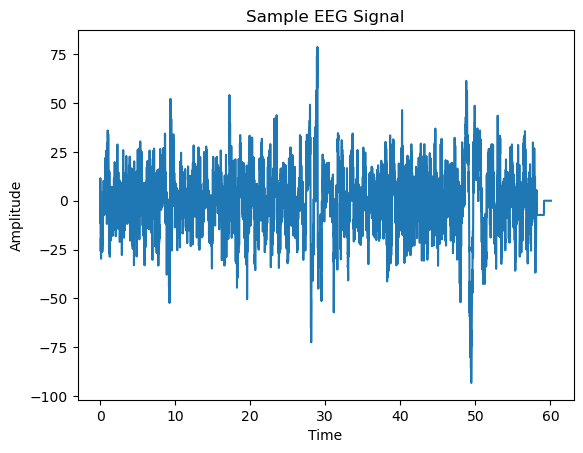
\includegraphics[width=0.4\textwidth]{figures/example_eeg.png}
        \caption{Example of EEG}
    \end{figure}
\end{frame}


\begin{frame}{Definition of the task}

    Objective : training a neural network that takes as an input a segment of 1000 points and outputs the probability for the patient to be currently performing a mental arithmetic task. \\[1cm]
    
    Structure : 
    \begin{enumerate}
        \item A first CNN to extract features from the EEG (vector  in $\mathbb{R}^{100}$). 
        \item A fully connected layer that outputs a probability to be in class 1. 
    \end{enumerate}

\end{frame}


\begin{frame}{Features Extractor}

    Based on StagerNet from \cite{banville2021uncovering}. 
    \begin{exampleblock}

        \begin{enumerate}
            \item 4 convolutional layers, padding = 1, kernel size = 3. 
            \item Dropout, relu activation function and max pool at each layer. 
            \item Last layer : fully connected. 
        \end{enumerate}
        
    \end{exampleblock}
    
\end{frame}


\begin{frame}{Pretraining}

    Pretraining of the feature extractor. \\

    Intuition: the features of two patterns from the same EEG should be the same if they are close in time. \\
    Training on 8928 pairs of subsequences close or not. \\
    Training on 100 epochs with BCE loss.\\
    
\end{frame}

\begin{frame}{Fine tuning}
    
    We added a fully connected layer and trained only the weights of the last layer on 200 epochs with BCE Loss on the dataset of EEG on the classification task. \\

    On the other hand, we trained the whole network not pretrained on the same dataset.

    Key points: 
    \begin{itemize}
        \item Clever initialization of the weights for the fully connected layer.
        \item Normalization of the EEG essential. 
    \end{itemize}
    
\end{frame}


\begin{frame}{Results}

    \begin{figure}
        \centering
        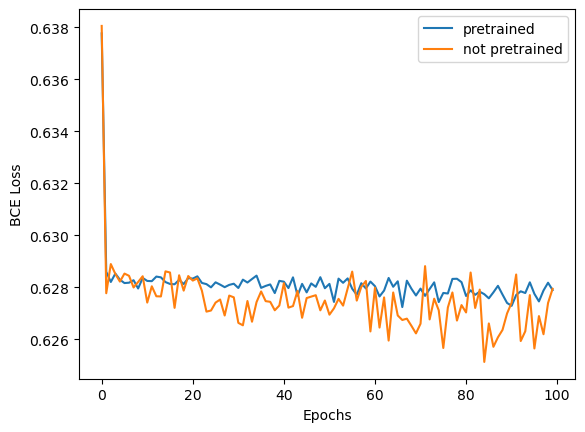
\includegraphics[width=0.4\textwidth]{figures/loss_train.png}
        \caption{Loss of the models during training }
    \end{figure}

    \begin{table}
        \centering
        \begin{tabular}{|c|c|c|}
            \hline
            Model & Test loss & F1 score \\
            \hline
            Pretrained & 0.62 & 0.81 \\
            \hline
            Not pretrained & 0.66 & 0.79 \\
            \hline
        \end{tabular}
        \caption{Results of the models}
    \end{table}

\end{frame}

\begin{frame}{Conclusion}

    \begin{itemize}
        \item Pretraining enables to get better results, especially when facing a small dataset.
        \item Other models could be tested, and different pretraining tasks could be tried. 
    \end{itemize}


\end{frame}



\begin{frame}
\printbibliography
\end{frame}


\end{document}
